\section{\textit{Autodesk Fusion 360}}
\label{sec:autodesk}

No desenvolvimento do modelo CAD do robô foram concebidas diversas peças: uma base, uma prateleira, uma tampa, uma bateria e quatro suportes. Para além destas peças, foram escolhidas peças já desenvolvidas: duas rodas motrizes, duas rodas giratórias, dois motores e doze sensores. Após todas as peças desenvolvidas e ajustadas, foi feito o assembler das diversas peças formando assim o robô. De seguida, é possível visualizar os desenhos técnicos de cada peça, a peça em modelo CAD e uma breve descrição de cada peça:

\begin{itemize}
    \item \emph{Base:} Projetou-se uma base cilíndrica com 1cm de altura e 15 cm de raio. Esta base serve de suporte a todo o robô e têm um encaixe para os motores (Figura \ref{fig:base}).
    %
    \begin{figure}[!h] 
\centering
    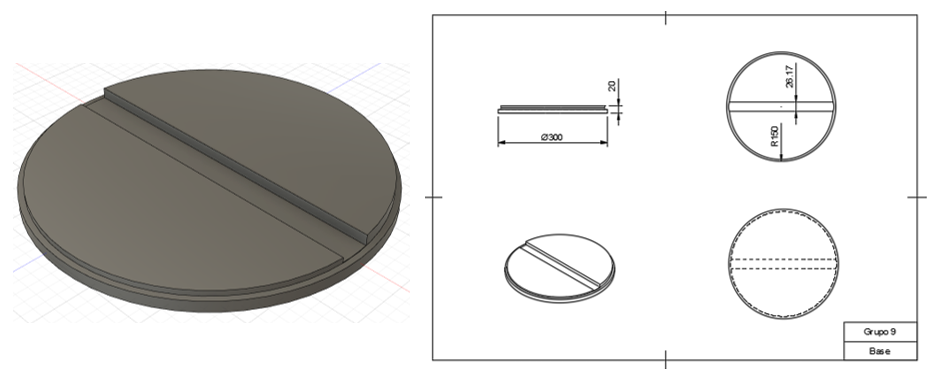
\includegraphics[width=0.7\textwidth]{./img/base}
  \caption{Base do robô}% 
\label{fig:base}
\end{figure}

    \item \emph{Prateleira:} Foi desenvolvida uma prateleira com 9 cm de altura, para criar duas divisões na base. Sendo a divisão inferior para a colocação dos motores e fios necessários e na divisão superior é colocada bateria. Esta prateleira serve para isolar todos os elementos que estão apoiados na base do exterior conferindo uma maior segurança dos mesmos (Figura \ref{fig:prateleira}).
    %
    \begin{figure}[!h] 
\centering
    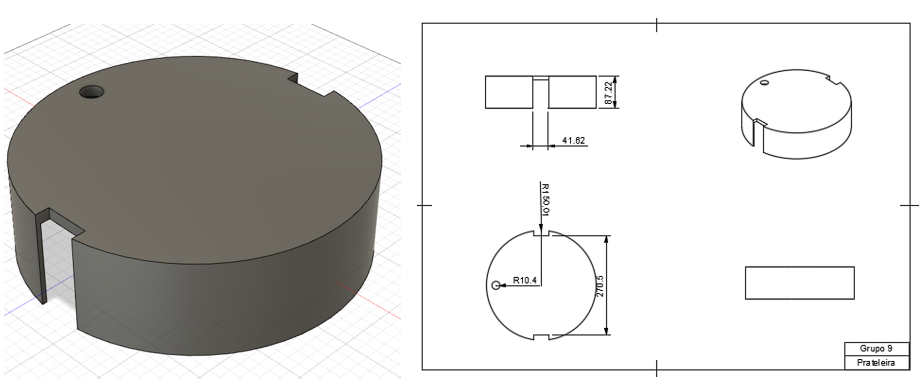
\includegraphics[width=0.65\textwidth]{./img/prateleira}
  \caption{Prateleira do robô}% 
\label{fig:prateleira}
\end{figure}

    \item \emph{Tampa:} Elaborou-se uma tampa com 2cm de altura e um raio de 15 cm, para que esta fique apoiada nos suportes. Esta tampa é a camada mais alta do robô e protege os elementos que estão abaixo dela (Figura \ref{fig:tampa}).
        %
    \begin{figure}[!h] 
\centering
    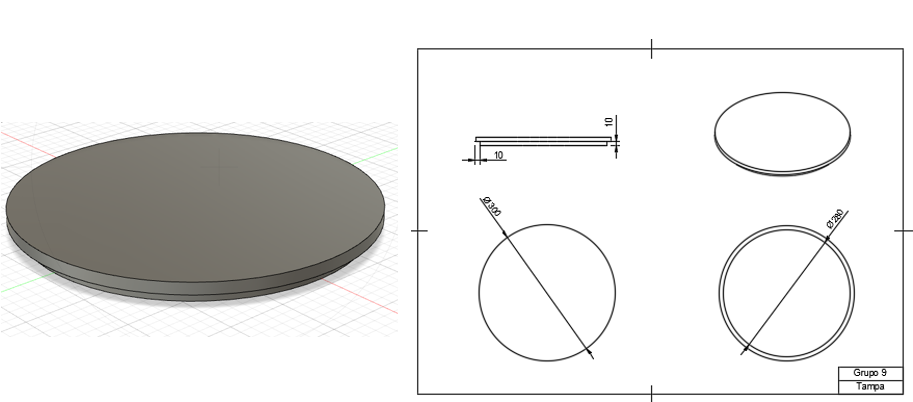
\includegraphics[width=0.65\textwidth]{./img/tampa}
  \caption{Tampa do robô}% 
\label{fig:tampa}
\end{figure}

\item \emph{Suportes:} Para dar altura ao robô de forma a colocar alguns elementos fora do interior do robô foram criados 4 suportes (Figura \ref{fig:suportes}).
        %
    \begin{figure}[!h] 
\centering
    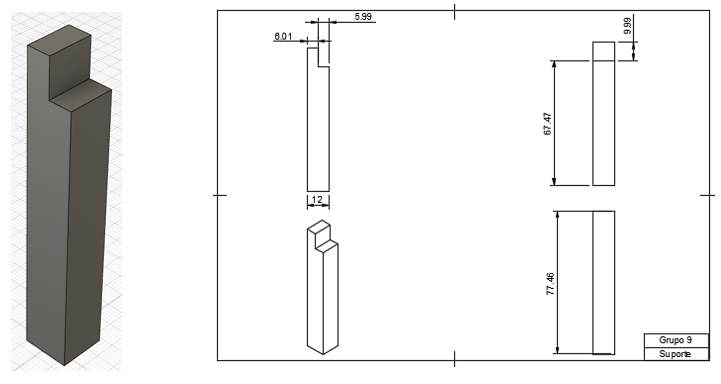
\includegraphics[width=0.6\textwidth]{./img/suportes}
  \caption{Suportes do robô}% 
\label{fig:suportes}
\end{figure}

\item \emph{Sensores:} O modelo do robô possui 12 sensores infravermelhos previamente concebidos, nos quais foi necessário ajustar as medidas. Estes estão igualmente espaçados entre si ao redor de toda a base. Estes sensores têm um alcance de 80 cm e uma amplitude de 30º (Figura \ref{fig:sensores-2}).
        %
    \begin{figure}[!h] 
\centering
    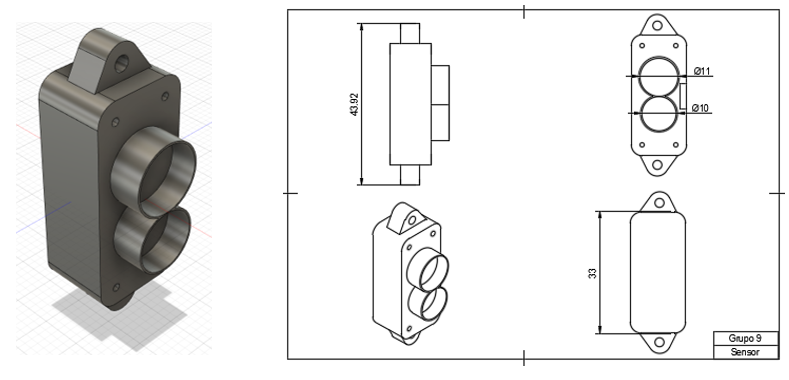
\includegraphics[width=0.6\textwidth]{./img/sensores-2}
  \caption{Sensores do robô}% 
\label{fig:sensores-2}
\end{figure}

\item \emph{Bateria:} : Foi desenvolvida uma bateria com 15 cm de comprimento, 10,5 cm de altura e 6,5 cm de largura. A bateria foi desenhada com base em modelos reais. Para fazer a bateria, foi desenhado um retângulo com 15 x 6,5 cm, utilizando a ferramenta \textit{Create Sketch}, de seguida, através da ferramenta extrude foi dada uma altura de 10,5 cm, conferindo-lhe assim a forma de paralelepípedo. Após isto feito, foi desenho um novo retângulo no topo do paralelepípedo e novamente através da ferramenta extrude foi removido o centro do retângulo de forma a criar os terminais que se encontram na parte de cima da bateria como é vísivel na figura seguinte (Figura \ref{fig:bateria}).
        %
    \begin{figure}[!h] 
\centering
    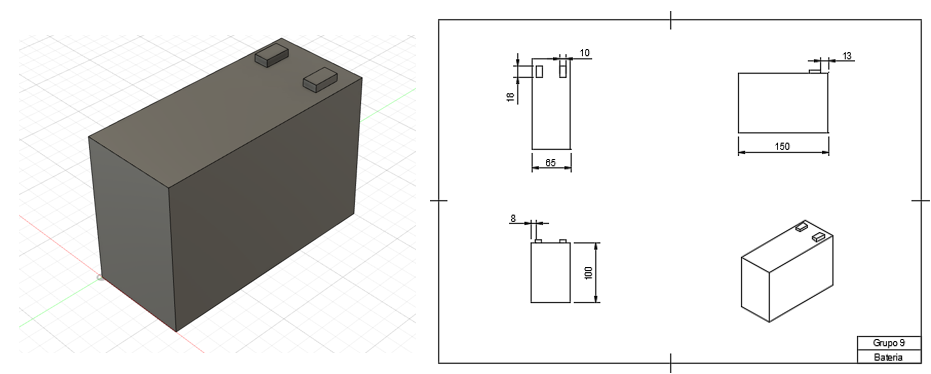
\includegraphics[width=0.8\textwidth]{./img/bateria}
  \caption{Bateria do robô}% 
\label{fig:bateria}
\end{figure}

\item \emph{Motor:} O modelo do robô possui dois motores 12V DC. Foi utilizado um design já concebido, sendo depois necessário adaptar às características do nosso robô (Figura \ref{fig:motor}).
        %
    \begin{figure}[!h] 
\centering
    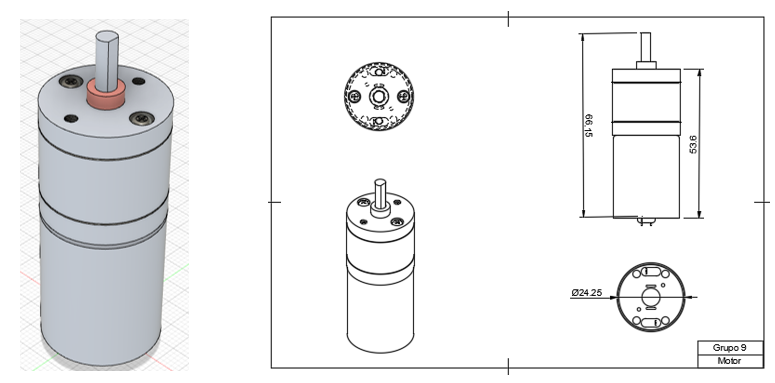
\includegraphics[width=0.6\textwidth]{./img/motor}
  \caption{Motores do robô}% 
\label{fig:motor}
\end{figure}

\item \emph{Rodas motriz e rodas giratórias:} O modelo do robô possui duas rodas motrizes e duas rodas giratórias. Foram utilizados designs já concebidos, sendo depois necessário adaptar às características do nosso robô (Figura \ref{fig:rodas-motriz} e Figura \ref{fig:rodas-gira}).
        %
    \begin{figure}[!h] 
\centering
    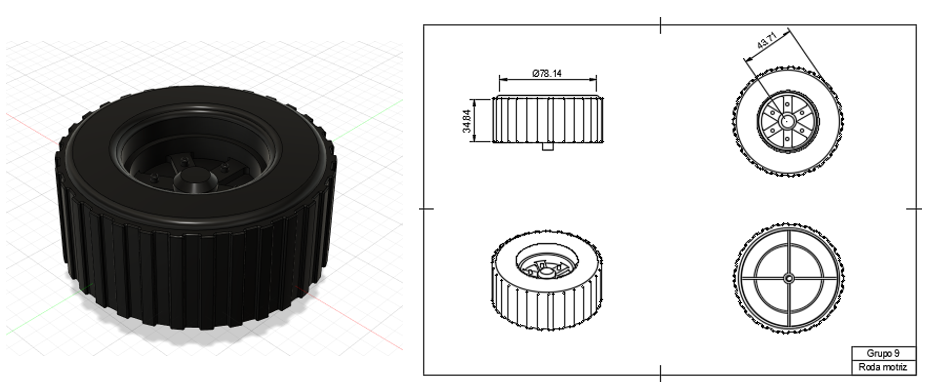
\includegraphics[width=0.6\textwidth]{./img/roda-motriz}
  \caption{Rodas motriz do robô}% 
\label{fig:rodas-motriz}
\end{figure}
        %
    \begin{figure}[!h] 
\centering
    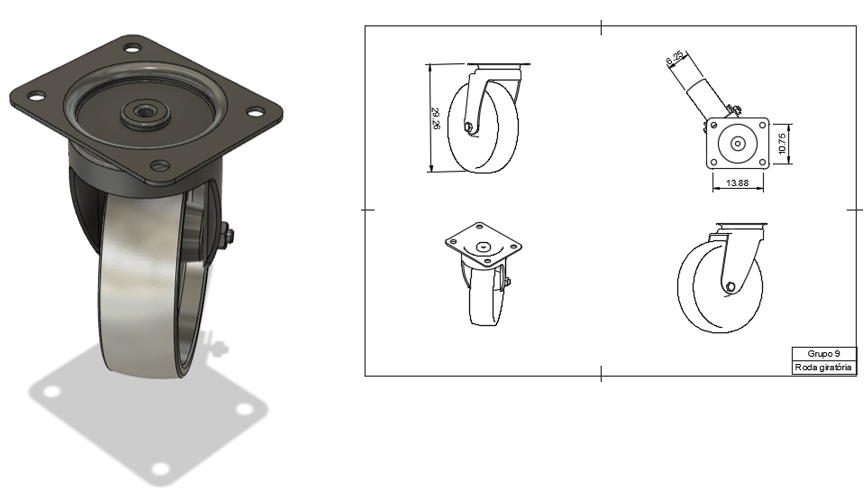
\includegraphics[width=0.6\textwidth]{./img/roda-gira}
  \caption{Rodas Giratórias do robô}% 
\label{fig:rodas-gira}
\end{figure}
\clearpage
\item \emph{Robô:} O robô é a junção de todas as peças mencionadas anteriormente (Figura \ref{fig:robo}).
        %
    \begin{figure}[!ht] 
\centering
    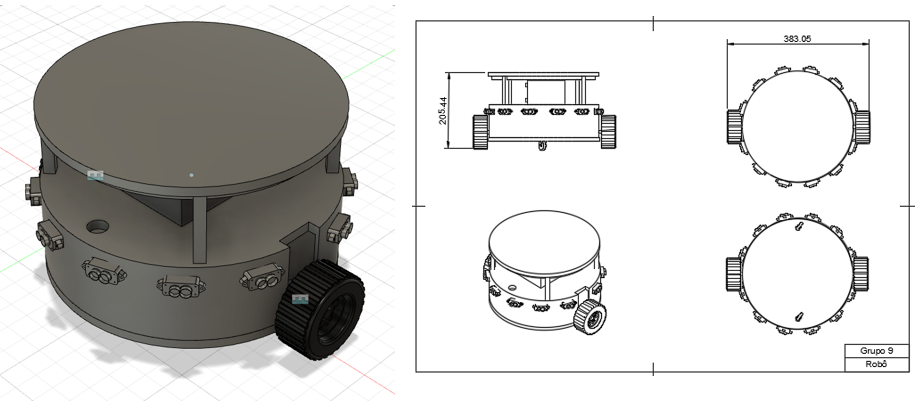
\includegraphics[width=0.7\textwidth]{./img/robo-total}
  \caption{Robô}% 
\label{fig:robo}
\end{figure}
\end{itemize}
\clearpage